\documentclass[border=0mm]{standalone}
\usepackage{fontspec}
\usepackage{xcolor}
\usepackage{unicode-math}
\usepackage{tikz}
\setmainfont{Linux Libertine O}
\setsansfont{Linux Biolinum O}
\usetikzlibrary{shapes.geometric}

\definecolor{mediumblue}{HTML}{0000CD}
\definecolor{green}{HTML}{008B00}

\newcommand{\mb}[1]{\textcolor{mediumblue}{#1}}
\newcommand{\gn}[1]{\textcolor{green}{#1}}

\begin{document}
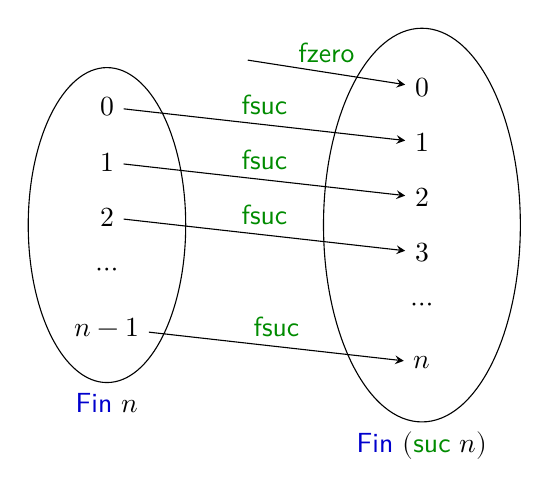
\begin{tikzpicture}[>=stealth]
    % First set (Fin n)
    \node[ellipse, draw, minimum width=2cm, minimum height=4cm] (finn) at (0,0) {};
    \node[below] at (finn.south) {$\mb{\mathsf{Fin}}\ n$};
    
    % Elements in Fin n
    \foreach \i in {0,...,2} {
        \node (n\i) at (0, 1.5 - \i*0.7) {$\i$};
    }
    \node at (0, 1.5 - 3*0.7) {$\cdots$};
    \node (nn) at (0, 1.5 - 4*0.7) {$n-1$};
    
    % Second set (Fin (suc n))
    \node[ellipse, draw, minimum width=2.5cm, minimum height=5cm] (finsucn) at (4,0) {};
    \node[below] at (finsucn.south) {$\mb{\mathsf{Fin}}\ (\gn{\mathsf{suc}}\ n)$};
    
    % Elements in Fin (suc n)
    \foreach \i in {0,...,3} {
        \node (s\i) at (4, 1.75 - \i*0.7) {$\i$};
    }
    \node at (4, 1.75 - 4*0.7) {$\cdots$};
    \node (sn) at (4, 1.75 - 5*0.7) {$n$};
    
    % Arrows (fsuc)
    \foreach \i [evaluate={\j=int(\i+1);}] in {0,...,2} {
        \draw[->] (n\i) -- (s\j) node[midway, above] {$\gn{\mathsf{fsuc}}$};
    }
    \draw[->] (nn) -- (sn) node[midway, above] {$\gn{\mathsf{fsuc}}$};
    
    % Arrow (fzero)
    \draw[->] ([xshift=-20mm, yshift=1mm]s0.north west) -- (s0) node[midway, above] {$\gn{\mathsf{fzero}}$};
\end{tikzpicture}
\end{document}